\newpage
\appendix
\onecolumn
\section{Appendix}

% =============================================================================
\subsection{Notation Summary}
\label{app:notation}

Table~\ref{tab:notation} summarizes the key notation used throughout the paper.

\begin{table}[h]
\caption{Summary of Notation}
\label{tab:notation}
\begin{center}
\begin{tabular}{cl}
\toprule
\textbf{Symbol} & \textbf{Description} \\
\midrule
\multicolumn{2}{l}{\textit{Request Parameters}} \\
$r_i$ & Request $i$ \\
$a_i$ & Arrival time of request $i$ \\
$n_i^{\text{in}}$ & Input token count of request $i$ \\
$n_i^{\text{out}}$ & Output token count of request $i$ (unknown at arrival) \\
$p_i$ & Processing time (latency) of request $i$ \\
$c_i$ & API cost of request $i$: $c_i = p^{\text{in}} n_i^{\text{in}} + p^{\text{out}} n_i^{\text{out}}$ \\
$m_i$ & Model type requested \\
\midrule
\multicolumn{2}{l}{\textit{Provider Parameters}} \\
$S_A$ & Pay-per-token API provider \\
$S_Q$ & Quota-based subscription provider \\
$S_C$ & Concurrency-limited subscription provider \\
$Q$ & Daily quota limit for $S_Q$ \\
$C$ & Concurrency limit for $S_C$ \\
$p^{\text{in}}, p^{\text{out}}$ & Price per input/output token (API) \\
\midrule
\multicolumn{2}{l}{\textit{Discretization (Stage 2 ILP)}} \\
$\Delta$ & Time slot size (seconds) \\
$\hat{p}_i$ & Processing time in slots: $\hat{p}_i = \lceil p_i / \Delta \rceil$ \\
$\alpha_i$ & Earliest feasible start slot for request $i$ on $S_C$ \\
$\beta_i$ & Latest feasible start slot for request $i$ on $S_C$ \\
$\ell$ & Max queueing delay in slots (0 = zero-wait/loss system) \\
\midrule
\multicolumn{2}{l}{\textit{Decision Variables}} \\
$x_i^A, x_i^Q, x_i^C$ & Binary routing decisions for request $i$ \\
$s_i$ & Start time of request $i$ on $S_C$ (conceptual; ILP uses $z_{i,t}$) \\
$z_{i,t}$ & Binary: request $i$ starts at time slot $t$ \\
\midrule
\multicolumn{2}{l}{\textit{Online Algorithm}} \\
$z = k/Q$ & Fraction of quota consumed \\
$\psi(z)$ & Shadow price (threshold) function \\
$L, U$ & Lower/upper bounds on request value \\
$\hat{v}_t$ & Estimated value of request at time $t$ \\
$\hat{L}_t^{(\tau)}$ & Predicted $\tau$-th quantile of output length \\
$\alpha$ & EMA smoothing factor \\
\midrule
\multicolumn{2}{l}{\textit{Metrics}} \\
CR & Competitive Ratio: $\text{Cost}_{\text{Online}} / \text{Cost}_{\text{Optimal}}$ \\
\bottomrule
\end{tabular}
\end{center}
\end{table}

% =============================================================================
\subsection{Stage 1: Proof of Optimality}
\label{app:stage1_proof}

We prove that the sorting-based algorithm is optimal for the Stage 1 quota allocation problem.

\begin{theorem}[Stage 1 Optimality]
For the fixed-window quota allocation problem with unit weights ($w_i = 1$), sorting requests by API cost in descending order and selecting the top-$Q$ requests is optimal.
\end{theorem}

\begin{proof}
Consider a single window with requests $\mathcal{R} = \{1, \ldots, n\}$ and quota $Q$. Let $c_i$ denote the API cost of request $i$. Without loss of generality, assume $c_1 \geq c_2 \geq \cdots \geq c_n$.

The sorting algorithm selects $S^* = \{1, 2, \ldots, \min(Q, n)\}$ with total savings $\sum_{i \in S^*} c_i$.

Suppose there exists an alternative solution $S'$ with $|S'| \leq Q$ and $\sum_{i \in S'} c_i > \sum_{i \in S^*} c_i$. Since $|S'| \leq Q = |S^*|$, there must exist some $j \in S^*$ such that $j \notin S'$, and some $k \notin S^*$ such that $k \in S'$.

By construction, $j \leq Q < k$, which implies $c_j \geq c_k$ (since costs are sorted in descending order). Consider the solution $S'' = (S' \setminus \{k\}) \cup \{j\}$. We have:
\[
\sum_{i \in S''} c_i = \sum_{i \in S'} c_i - c_k + c_j \geq \sum_{i \in S'} c_i
\]

By repeatedly applying this exchange argument, we can transform any solution into $S^*$ without decreasing the objective. Therefore, $S^*$ is optimal.
\end{proof}

\paragraph{Complexity.} The algorithm runs in $O(n \log n)$ time due to sorting, where $n$ is the number of requests per window.

\paragraph{Extension to Variable Weights.} When $w_i$ varies (e.g., token-based quotas), the problem becomes a 0/1 knapsack instance, which is NP-hard. In this case, we use dynamic programming or ILP solvers.

% =============================================================================
\subsection{Stage 2: NP-Hardness}
\label{app:stage2_hardness}

We prove that the Stage 2 problem (joint quota and concurrency optimization) is NP-hard by
reduction from the $0/1$ knapsack problem.

\begin{theorem}[Stage 2 NP-Hardness]
The Stage 2 routing problem is NP-hard, even in the special case with no quota ($Q=0$),
unit concurrency weights ($w_i=1$), a single concurrency slot ($C=1$), and identical arrival
times ($a_i=0$ for all requests).
\end{theorem}

\begin{proof}
We reduce from the $0/1$ knapsack problem. A knapsack instance consists of items
$i \in \{1,\dots,n\}$, each with a size $\omega_i \in \mathbb{Z}_{>0}$ and a value
$v_i \in \mathbb{Z}_{>0}$, and a capacity $W \in \mathbb{Z}_{>0}$. The goal is to select
a subset $S$ that maximizes $\sum_{i \in S} v_i$ subject to $\sum_{i \in S} \omega_i \le W$.

\textbf{Construction.} Given a knapsack instance, construct a Stage 2 instance for a single day
with the following settings:
\begin{itemize}
    \item Disable $S_Q$ by setting $Q=0$.
    \item Set concurrency limit $C=1$ and weights $w_i=1$ (one slot per request).
    \item Fix a common completion deadline $d_i = W$ for all requests and set $a_i=0$.
    \item For each item $i$, create a request with processing time $p_i = \omega_i$ and API cost
          $c_i = v_i$.
\end{itemize}
Routing a request to $S_C$ yields zero marginal cost; routing to the API incurs cost $c_i$.

\textbf{Equivalence.} Since $C=1$ and all arrivals are at time $0$, a set of requests can be
scheduled on $S_C$ and completed by time $W$ if and only if
$\sum_{i \in S} p_i \le W$. The Stage 2 objective minimizes total API cost
\[
\sum_{i \notin S} c_i = \sum_{i=1}^n c_i - \sum_{i \in S} c_i,
\]
which is equivalent to maximizing the avoided API cost $\sum_{i \in S} c_i$ subject to the
same capacity constraint. This is exactly the knapsack objective with values $v_i=c_i$ and
sizes $\omega_i=p_i$. Therefore, Stage 2 is NP-hard.
\end{proof}

\paragraph{Practical Implications.} Despite NP-hardness, our ILP formulation (Section~\ref{app:stage2_ilp}) can solve instances with thousands of requests within minutes using modern solvers like Gurobi. The time-indexed formulation exploits the structure of the problem, and preprocessing (e.g., fixing obvious routing decisions) further reduces solve time.

% =============================================================================
\subsection{Stage 2: ILP Formulation}
\label{app:stage2_ilp}

We provide the complete time-indexed ILP formulation for Stage 2 with both quota and concurrency constraints.

\paragraph{Decision Variables.}
\begin{itemize}
    \item $x_i^Q \in \{0, 1\}$: request $i$ is served by quota-based subscription $S_Q$
    \item $x_i^C \in \{0, 1\}$: request $i$ is served by concurrency-limited subscription $S_C$
    \item $x_i^A \in \{0, 1\}$: request $i$ is served by API $S_A$
    \item $z_{i,t} \in \{0, 1\}$: request $i$ starts on $S_C$ at time slot $t$
\end{itemize}

\paragraph{Parameters.}
\begin{itemize}
    \item $a_i$: arrival time of request $i$
    \item $p_i$: processing time of request $i$
    \item $c_i$: API cost of request $i$
    \item $Q$: daily quota for $S_Q$
    \item $C$: concurrency limit for $S_C$
    \item $w_i$: weight (GPU slots) consumed by request $i$ on $S_C$
    \item $\Delta$: time slot size (seconds)
    \item $\ell$: maximum queueing delay (in slots), with $\ell=0$ for a zero-wait system
\end{itemize}

\paragraph{Objective.} Minimize total API cost:
\[
\min \sum_{i} c_i \cdot x_i^A
\]

\paragraph{Time Discretization.}
We discretize time into slots $t \in \{0, 1, \dots, T\}$ with slot width $\Delta$. Let
$\hat{p}_i = \lceil p_i/\Delta \rceil$ be the processing time in slots and let
$\alpha_i = \lceil a_i/\Delta \rceil$ be the earliest feasible start slot. Under a bounded
queueing model (used in our experiments), a request assigned to $S_C$ may start at any slot
$t \in [\alpha_i, \beta_i]$ where $\beta_i = \alpha_i + \ell$. If a hard completion deadline
$d_i$ exists, we can further restrict $\beta_i \le \lfloor d_i/\Delta \rfloor - \hat{p}_i$.

\paragraph{Constraints.}
\begin{align}
& x_i^Q + x_i^C + x_i^A = 1 && \forall i \in \mathcal{R} \tag{Assignment} \\
& \sum_{i \in \mathcal{R}_d} x_i^Q \leq Q && \forall d \in \mathcal{D} \tag{Daily Quota} \\
& \sum_{t=\alpha_i}^{\beta_i} z_{i,t} = x_i^C && \forall i \in \mathcal{R} \tag{Start Time} \\
& \sum_{i \in \mathcal{R}} w_i \sum_{\tau=\max(\alpha_i,\, t-\hat{p}_i+1)}^{\min(\beta_i,\, t)} z_{i,\tau} \le C
&& \forall t \in \{0,\dots,T\} \tag{Concurrency}
\end{align}

The start-time constraint chooses exactly one start slot for each request routed to $S_C$.
The concurrency constraint counts all requests whose chosen start time implies they are active
at slot $t$, enforcing that the total active weight never exceeds $C$.

\paragraph{Zero-Wait Semantics.} In the zero-wait (loss) system, requests cannot queue. This is
captured by setting $\ell=0$, so $\beta_i=\alpha_i$ and each request assigned to $S_C$ must
start immediately upon arrival.

% =============================================================================
\subsection{Primal-Dual Algorithm Analysis}
\label{app:primal_dual}

\textbf{Threshold Function.}
The shadow price (threshold) function for the quota constraint is:
\[
\psi(z) = L \cdot \left(\frac{U}{L}\right)^z
\]
where $z = k/Q$ is the fraction of quota consumed, $L$ is the lower bound on request values (e.g., 5th percentile), and $U$ is the upper bound on request values (e.g., 95th percentile).

\textbf{Intuition.} The threshold starts at $L$ (low bar when quota is abundant) and grows exponentially to $U$ as quota depletes. This ensures that early requests with moderate value are accepted, while late requests must have high value to justify consuming scarce quota.

\textbf{Competitive Ratio.}
\begin{samepage}
\begin{theorem}
The primal-dual algorithm achieves a competitive ratio of $O(\ln(U/L))$ for the online knapsack problem with known values.
\end{theorem}
\begin{proof}[Proof Sketch]
The proof follows from the online primal-dual framework. The threshold function $\psi(z)$ corresponds to the dual variable for the capacity constraint. The exponential form ensures that the total dual cost grows proportionally to the primal objective, yielding the logarithmic competitive ratio.
\end{proof}
\end{samepage}

\textbf{Practical Considerations.}
In practice, request values are not known exactly at arrival time (output tokens are unknown). We use EMA-based estimates, which introduces prediction error. The competitive ratio guarantee holds for the estimated values; actual performance depends on prediction quality.

% =============================================================================
\Needspace{24\baselineskip}
\subsection{Learning-Augmented Algorithm (LA-PD)}
\label{app:lapd}

\noindent\textbf{Algorithm Pseudocode.} Algorithm~\ref{alg:app_lapd} provides the pseudocode for the learning-augmented primal-dual (LA-PD) rule.

\begin{algorithm}[H]
\caption{Learning-Augmented Primal-Dual Routing (LA-PD)}
\label{alg:app_lapd}
\begin{algorithmic}[1]
\STATE \textbf{Input:} Request $r_t$ with features $\mathbf{x}_t$, quota usage $k_t$, concurrency state
\STATE \textbf{Parameters:} Quota $Q$, concurrency $C$, value bounds $[L, U]$, predictor $\mathcal{M}$
\STATE \textcolor{gray}{// Step 1: Get quantile predictions for output length}
\STATE $\hat{L}_t^{(10)}, \hat{L}_t^{(50)}, \hat{L}_t^{(90)} \gets \mathcal{M}.\text{predict}(\mathbf{x}_t)$
\STATE \textcolor{gray}{// Step 2: Compute conservative value estimate (LCB)}
\STATE $\hat{v}_t^{\text{LCB}} \gets (n_t^{\text{in}} \cdot p^{\text{in}} + \hat{L}_t^{(10)} \cdot p^{\text{out}}) / 1000$
\STATE \textcolor{gray}{// Step 3: Estimate processing duration (UCB)}
\STATE $\hat{p}_t \gets \widehat{\text{TTFT}}^{(90)} + \hat{L}_t^{(90)} / \widehat{\text{TPS}}^{(10)}$
\STATE \textcolor{gray}{// Step 4: Compute shadow prices}
\STATE $z_t \gets k_t / Q$; \quad $\psi_t \gets L \cdot (U/L)^{z_t}$
\STATE $\lambda_t \gets$ CongestionPrice(concurrency state) \textcolor{gray}{// See Eq.~(2) in main text}
\STATE \textcolor{gray}{// Step 5: Compute net gains for each option}
\STATE $G_Q \gets \hat{v}_t^{\text{LCB}} - \psi_t$; \quad $G_C \gets \hat{v}_t^{\text{LCB}} - \lambda_t \cdot w_t \cdot \hat{p}_t$; \quad $G_A \gets 0$
\STATE \textcolor{gray}{// Step 6: Apply capacity constraints}
\IF{$k_t \geq Q$}
    \STATE $G_Q \gets -\infty$
\ENDIF
\IF{model $m_t$ not supported by $S_C$}
    \STATE $G_C \gets -\infty$
\ENDIF
\STATE \textcolor{gray}{// Step 7: Risk-aware routing decision}
\IF{$G_Q \geq G_C$ \AND $G_Q > 0$}
    \STATE \textbf{return} $S_Q$; update $k_{t+1} \gets k_t + 1$
\ELSIF{$G_C > 0$}
    \STATE \textbf{return} $S_C$; update concurrency state
\ELSE
    \STATE \textbf{return} $S_A$ (API)
\ENDIF
\end{algorithmic}
\end{algorithm}

\paragraph{Key Design Choices.}
\begin{enumerate}
    \item \textbf{P10 for Value Estimation:} Using the 10th percentile provides a conservative lower bound, avoiding the "winner's curse" of routing low-value requests that appear high-value due to prediction noise.
    \item \textbf{Safeguard Mechanism:} When predictions are suspiciously low ($< \epsilon$), we fall back to EMA-based estimates to maintain robustness.
    \item \textbf{No Explicit $\lambda$ Tuning:} Unlike heuristics like $\hat{v} - \lambda\sigma$, directly using predicted quantiles provides uncertainty without introducing an additional tuning parameter.
\end{enumerate}

% =============================================================================
\subsection{Predictor Details}
\label{app:predictors}

\paragraph{EMA Predictor.}
The Exponential Moving Average predictor maintains a running estimate of output length:
\[
\hat{L}_{t+1} = \alpha \cdot L_t^{\text{actual}} + (1 - \alpha) \cdot \hat{L}_t
\]
where $\alpha \in (0, 1)$ controls the smoothing factor (we use $\alpha = 0.1$).

\textbf{Pros:} Simple, no training required, adapts to distribution shift.\\
\textbf{Cons:} Single point estimate, no uncertainty quantification.

\paragraph{Histogram Predictor.}
The histogram predictor maintains empirical quantiles of output length, bucketed by input length ranges:
\begin{enumerate}
    \item Partition input length into bins: $[0, 100), [100, 500), [500, 2000), \ldots$
    \item For each bin, maintain a rolling histogram of output lengths (last 1000 samples)
    \item At prediction time, return the $\tau$-th percentile from the appropriate bin
\end{enumerate}

\textbf{Pros:} Provides calibrated quantile estimates, captures input-output correlation.\\
\textbf{Cons:} Requires sufficient samples per bin, may lag during distribution shift.

\Needspace{18\baselineskip}
\noindent\textbf{EMA Predictor Pseudocode.} Algorithm~\ref{alg:app_ema_predictor} summarizes the EMA baseline used in our experiments.

\begin{algorithm}[H]
\caption{Exponential Moving Average (EMA) Predictor}
\label{alg:app_ema_predictor}
\begin{algorithmic}
\STATE \textbf{Initialize:} $\hat{L} \gets L_{\text{default}}$ (e.g., 500 tokens)
\STATE \textbf{Parameter:} $\alpha = 0.1$ (smoothing factor)
\STATE \textbf{function} Predict($r_t$):
\STATE \quad \textbf{return} $\hat{L}$
\STATE \textbf{function} Update($r_t$, $L_t^{\text{actual}}$):
\STATE \quad $\hat{L} \gets \alpha \cdot L_t^{\text{actual}} + (1 - \alpha) \cdot \hat{L}$
\end{algorithmic}
\end{algorithm}

\Needspace{22\baselineskip}
\noindent\textbf{Histogram Predictor Pseudocode.} Algorithm~\ref{alg:app_hist_predictor} summarizes the histogram-based quantile predictor baseline.

\begin{algorithm}[H]
\caption{Histogram-based Quantile Predictor}
\label{alg:app_hist_predictor}
\begin{algorithmic}
\STATE \textbf{Initialize:} Bins $\mathcal{B} = \{[0, 100), [100, 500), [500, 2000), [2000, \infty)\}$
\STATE \textbf{Initialize:} For each bin $b$, history $H_b \gets []$ (max size 1000)
\STATE \textbf{Parameter:} Quantile $\tau$ (e.g., 0.10 for P10)
\STATE \textbf{function} Predict($r_t$):
\STATE \quad $b \gets \text{GetBin}(n_t^{\text{in}})$
\IF{$|H_b| < 10$}
    \STATE \quad \textbf{return} $L_{\text{default}}$
\ENDIF
\STATE \quad Sort $H_b$ and \textbf{return} $\tau$-th percentile
\STATE \textbf{function} Update($r_t$, $L_t^{\text{actual}}$):
\STATE \quad $b \gets \text{GetBin}(n_t^{\text{in}})$
\STATE \quad Append $L_t^{\text{actual}}$ to $H_b$
\IF{$|H_b| > 1000$}
    \STATE \quad Remove oldest entry from $H_b$
\ENDIF
\end{algorithmic}
\end{algorithm}

% =============================================================================
\subsection{Duration Estimation Details}
\label{app:duration}

For concurrency-aware routing ($S_C$), we need to estimate the processing time $\hat{p}_t$ of each request to compute the occupancy cost $\lambda_t \cdot w_t \cdot \hat{p}_t$. Underestimating duration leads to optimistic slot occupancy assumptions, causing over-admission and queue buildup.

\paragraph{Decomposition.} We decompose the total latency into time-to-first-token (TTFT) and decode time:
\begin{equation}
    p_t = \text{TTFT}_t + \frac{n_t^{\text{out}}}{\text{TPS}_t}
\end{equation}
where TPS is the decode throughput (tokens per second). Both TTFT and TPS vary with server load, model, and request complexity.

\paragraph{Upper Confidence Bound (UCB) Estimation.} To avoid underestimating slot occupancy, we use conservative (pessimistic) estimates:
\begin{itemize}
    \item \textbf{TTFT:} Use the 90th percentile from recent history, $\widehat{\text{TTFT}}^{(90)}$
    \item \textbf{Output length:} Use the 90th percentile prediction, $\hat{L}_t^{(90)}$
    \item \textbf{TPS:} Use the 10th percentile from recent history, $\widehat{\text{TPS}}^{(10)}$ (lower TPS = longer decode time)
\end{itemize}

The UCB duration estimate is:
\begin{equation}
    \hat{p}_t^{\text{UCB}} = \widehat{\text{TTFT}}^{(90)} + \frac{\hat{L}_t^{(90)}}{\widehat{\text{TPS}}^{(10)}}
\end{equation}

\paragraph{Practical Implementation.} We maintain rolling windows (last 100 requests) for TTFT and TPS statistics, stratified by model. For new models with insufficient history, we use conservative defaults (TTFT = 2s, TPS = 20 tokens/s for 70B models).

\paragraph{Calibration Analysis.} On our Enterprise dataset, the UCB estimate achieves 92\% coverage (actual duration $\leq$ estimate in 92\% of cases), compared to 48\% coverage for point estimates. This conservative bias is intentional: it is better to occasionally route to API than to over-commit $S_C$ capacity.

% =============================================================================
\subsection{Dataset Statistics}
\label{app:datasets}

\begin{table}[h]
\caption{Extended Dataset Statistics}
\label{tab:datasets_extended}
\begin{center}
\begin{tabular}{lccccc}
\toprule
Dataset & Requests & Days & Models & Avg In & Avg Out \\
\midrule
ShareGPT & 201,318 & 7 & 1 & 156 & 423 \\
FreeInference & 371,214 & 90 & 12 & 892 & 1,247 \\
Enterprise & 54,599 & 84 & 8 & 2,341 & 3,892 \\
BurstGPT & 1,423,847 & 61 & 1 & 234 & 512 \\
\bottomrule
\end{tabular}
\end{center}
\end{table}

\paragraph{Workload Characteristics.}
\begin{itemize}
    \item \textbf{ShareGPT:} Standard chatbot workload with moderate output lengths.
    \item \textbf{FreeInference:} Diverse API gateway with multi-model mix. High variance in both input and output.
    \item \textbf{Enterprise:} Anonymized workload from a coding assistant deployment with long contexts. Highest cost variance (CV > 2).
    \item \textbf{BurstGPT:} Large-scale synthetic trace for online algorithm evaluation.
\end{itemize}

% =============================================================================
\subsection{Ablation Study: Predictor vs Decision Rule}
\label{app:ablation}

We conduct a 2x2 ablation study to disentangle the contributions of the predictor and the decision rule.

\begin{table}[h]
\caption{2x2 Ablation: Competitive Ratio (lower is better)}
\label{tab:ablation_extended}
\begin{center}
\begin{tabular}{lcc}
\toprule
 & EMA Predictor & Histogram Predictor \\
\midrule
Primal-Dual & \textbf{1.18} & 1.19 \\
LA-PD (P10) & 1.19 & 1.21 \\
\bottomrule
\end{tabular}
\end{center}
\end{table}

\paragraph{Key Finding.} Predictor quality matters more than decision rule complexity. The simple EMA predictor with Primal-Dual achieves the best competitive ratio (1.18), outperforming the more sophisticated histogram predictor. This suggests that for routing decisions, a responsive point estimate is more valuable than calibrated quantiles when the underlying distribution shifts frequently.

% =============================================================================
\subsection{Fixed-Window vs Rolling-Window Assumption}
\label{app:window}

A key modeling assumption in our Stage 1 analysis is the use of \textbf{fixed (disjoint) time windows} rather than rolling windows. We discuss this assumption in detail.

\paragraph{Real-World Rate Limits.}
Most commercial LLM subscriptions enforce rolling-window rate limits. For example, ChatGPT Plus allows approximately 80 messages per 3-hour rolling window, meaning at any time $t$, the user can send at most 80 messages in the interval $[t-3h, t]$. Similarly, Claude Pro and API tier limits use rolling windows.

\paragraph{Our Approximation.}
We approximate rolling windows with \textbf{fixed, disjoint windows} aligned to a reference time $t_0$. For a window length $W$ (e.g., 3 hours), we define window $k$ as the interval $[t_0 + kW, t_0 + (k+1)W)$. The quota $Q$ resets at each window boundary.

\paragraph{Why Fixed Windows?}
Fixed windows enable a \textbf{closed-form optimal solution}: within each window, the problem decomposes into independent knapsack instances that can be solved by sorting. Rolling windows create temporal dependencies across time that make the offline problem significantly more complex (the optimal solution at time $t$ depends on decisions made in $[t-W, t]$).

\paragraph{Lower Bound Property.}
Fixed windows are \textbf{strictly less restrictive} than rolling windows. Consider a burst of $2Q$ requests arriving at a window boundary: under fixed windows, $Q$ can be served in the ending window and $Q$ in the starting window; under rolling windows, only $Q$ can be served in any 3-hour span. Therefore, our Stage 1 oracle provides an \textbf{optimistic lower bound} on the achievable API cost under true rolling-window constraints.

\paragraph{Practical Implications.}
\begin{itemize}
    \item Our reported ``Optimal'' savings are upper bounds on what is achievable in practice.
    \item The gap between our oracle and a rolling-window oracle depends on workload burstiness at window boundaries. For smooth arrival patterns, the gap is small.
    \item Online algorithms (which make decisions without future knowledge) are unaffected by this distinction, as they cannot exploit window boundaries anyway.
\end{itemize}

% =============================================================================
\subsection{Real-World Subscription Plans}
\label{app:plans}

Here we map real-world subscription plans to our framework.

\textbf{OpenAI / Anthropic (Tier-based).} These providers use rolling-window rate limits (e.g., ``80 messages per 3 hours'' for ChatGPT Plus, ``45 messages per 5 hours'' for Claude Pro).
\begin{itemize}
    \item \textbf{Mapping:} We use fixed windows of the same duration as the rolling window. As discussed in Appendix~\ref{app:window}, this provides a lower bound on cost.
\end{itemize}

\textbf{Chutes.ai / Dedicated Endpoints.} These providers offer "throughput-based" pricing, which maps directly to our Stage 2 ($S_C$) concurrency constraint.
\begin{itemize}
    \item \textbf{Mapping:} A dedicated GPU instance (e.g., H100) provides a fixed number of concurrent slots $C$. The "quota" is effectively infinite, but throughput is bounded.
\end{itemize}

\textbf{Coding Copilots (e.g., Cursor, GitHub Copilot).} These often have "fast" and "slow" pools.
\begin{itemize}
    \item \textbf{Mapping:} The "fast pool" corresponds to our $S_Q$ (limited high-priority quota). The "slow pool" can be modeled as a high-latency fallback or a separate $S_C$ with lower priority.
\end{itemize}

% =============================================================================
\subsection{Multi-Model Routing}
\label{app:multimodel}

Our framework naturally extends to multi-model scenarios where a single subscription covers multiple models (e.g., an "All-Access" plan).

\textbf{Shared Quota.} If multiple models $m_1, m_2$ share a single quota $Q$, the Primal-Dual algorithm works unchanged. The shadow price $\psi(z)$ reflects the opportunity cost of the \textit{shared} resource. A request for $m_1$ is routed to subscription if its specific avoided cost $v_{t, m_1}$ exceeds $\psi(z)$. This automatically prioritizes expensive models (e.g., GPT-4) over cheap ones (e.g., GPT-3.5) for the shared quota.

\textbf{Separate Quotas.} If models have independent quotas $Q_1, Q_2$, we simply maintain separate state variables $z_1, z_2$ and thresholds $\psi_1(z_1), \psi_2(z_2)$.

% =============================================================================
\subsection{Latency-Constrained Optimization}
\label{app:latency}

While our main formulation focuses on cost, latency is a critical constraint. We can extend our ILP and Online algorithms to handle hard deadlines.

\textbf{Hard Deadlines.} In Stage 2 ILP, we enforce $s_i + p_i \le d_i$. If a request cannot be scheduled on $S_C$ by its deadline, it must be routed to $S_A$ (assuming $S_A$ meets the SLO).

\textbf{Soft Deadlines (Hedging).} For online routing, we can employ a hedging strategy: send a request to $S_C$ first, and if it is not completed by time $t_{hedge}$, speculatively send a backup request to $S_A$. The cost function then becomes the expected cost of the combined policy.

\begin{figure}[h]
\begin{center}
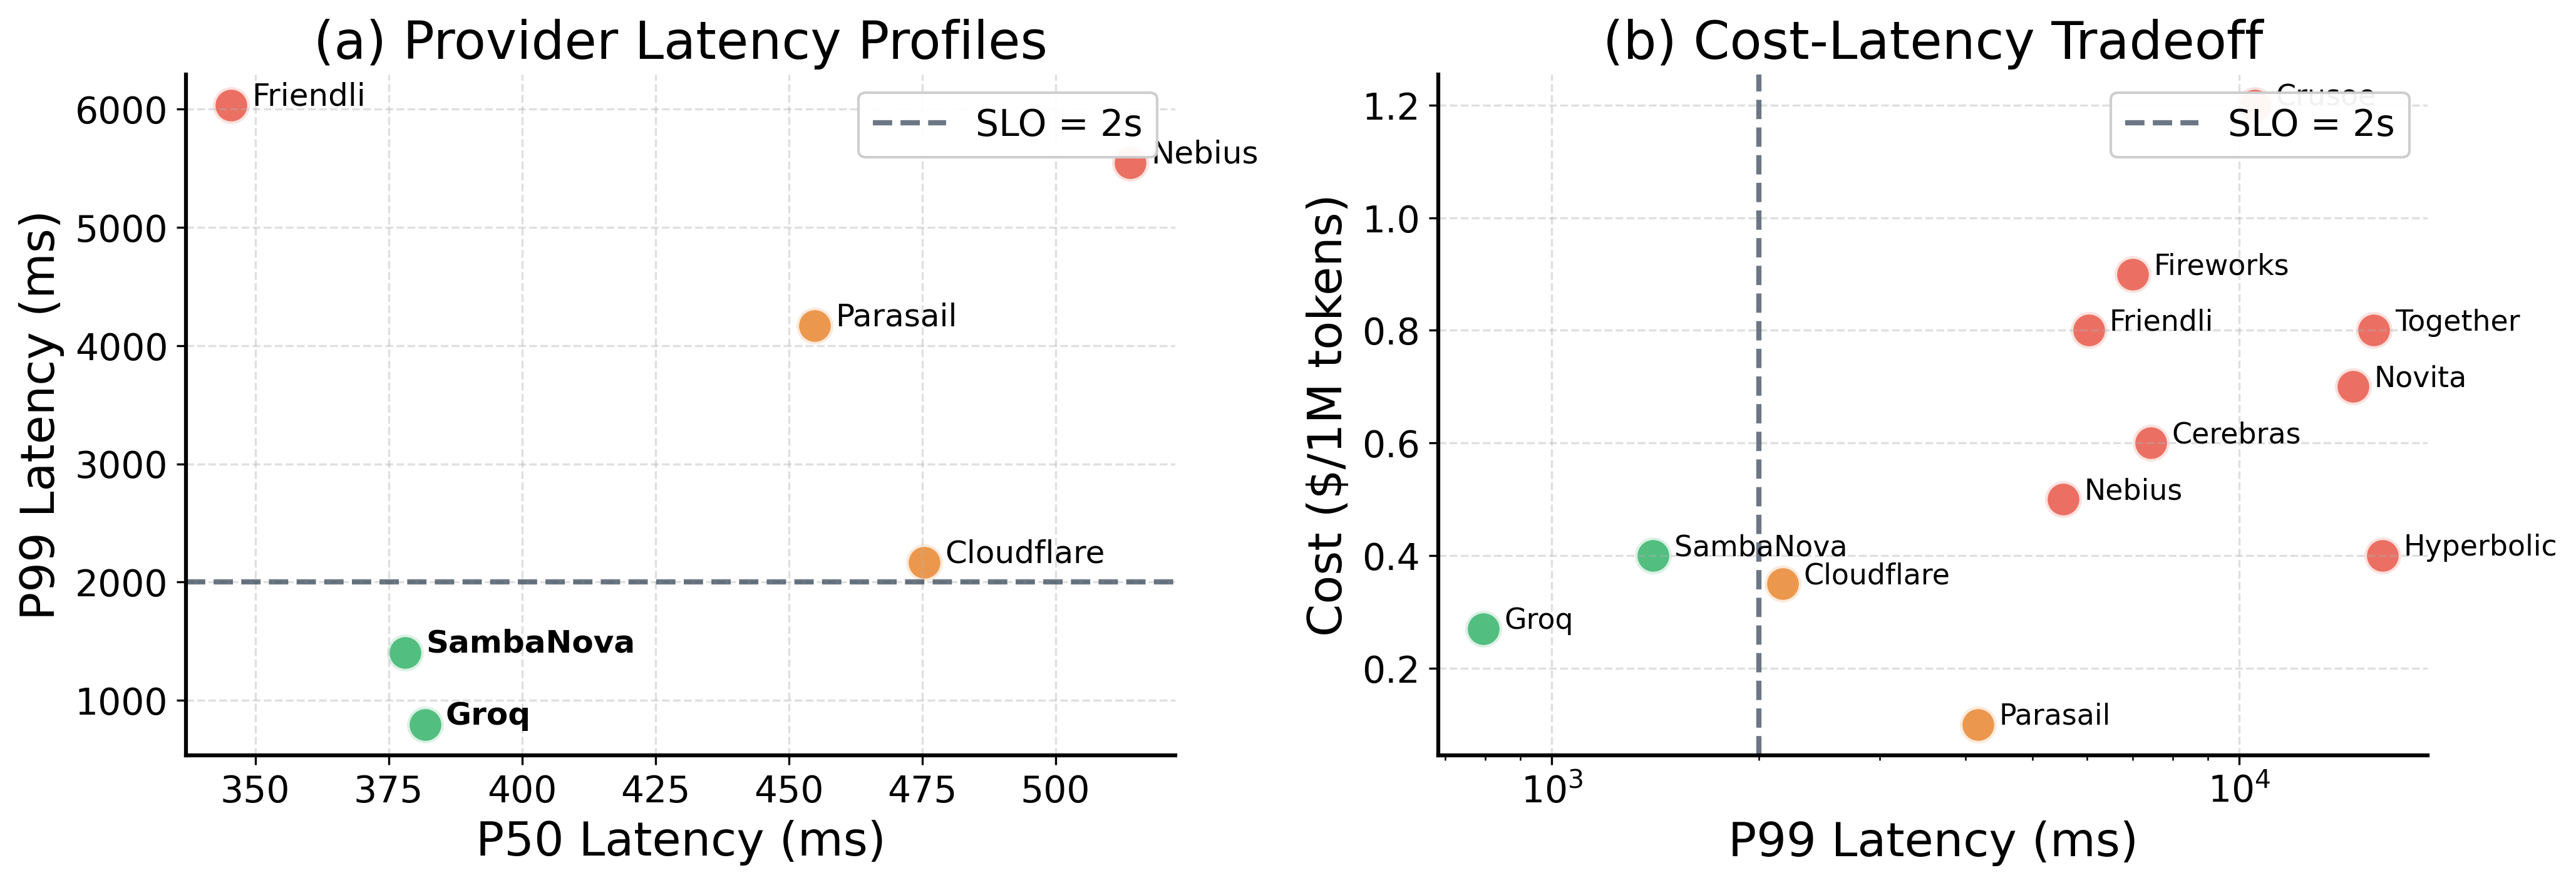
\includegraphics[width=0.9\textwidth]{images/latency_pareto_openrouter.png}
\caption{Provider latency profiles on OpenRouter (Llama-3.3-70B-Instruct). (a) P50 vs P99 latency showing provider reliability. (b) Cost-latency tradeoff---fast providers (Groq, SambaNova) meet tight SLOs but cost more; slower providers offer savings when SLOs are relaxed.}
\label{fig:latency_pareto}
\end{center}
\end{figure}

\paragraph{Online Latency Evaluation Setup.}
\label{app:latency_eval_setup}

We evaluate our latency-aware routing on the OpenRouter platform, which provides access to the same model (Llama-3.3-70B-Instruct) across 12+ providers with different latency and cost profiles.

\textbf{Model and Workload.} We use \texttt{meta-llama/llama-3.3-70b-instruct} served via OpenRouter. The workload combines BurstGPT arrival timestamps (realistic request patterns) with ShareGPT prompts (real user queries), replayed over 24 hours.

\textbf{Policies Compared.} We evaluate the following routing strategies:
\begin{itemize}
    \item \textbf{OpenRouter Auto}: OpenRouter's default routing (baseline). We do not specify a provider, allowing OpenRouter to select automatically.
    \item \textbf{Fastest Fixed}: Always route to the fastest provider (Groq) regardless of cost.
    \item \textbf{Cheapest Fixed}: Always route to the cheapest provider (Parasail) regardless of latency.
    \item \textbf{LP-Mix}: Our LP-based provider mixing (Section~\ref{sec:latency}) that constructs a cost-latency Pareto-optimal distribution over providers.
    \item \textbf{Smart Hedge}: LP-Mix as primary routing, with survival-analysis-based hedging (Eq.~\ref{eq:hedge_survival}) that triggers a backup request to the fastest provider when the primary exceeds its P90 latency threshold.
\end{itemize}

\textbf{Fairness Protocol.} To ensure fair comparison, each trace request is sent to \emph{all} policies simultaneously. This guarantees that all policies experience identical network conditions and provider load for the same request, enabling direct comparison of routing decisions.

\textbf{SLO Definition.} We define the latency SLO as Time-To-First-Token (TTFT) $\le$ 2 seconds. A request violates the SLO if TTFT exceeds 2s or the request fails.

\paragraph{Cancel-Aware Cost Analysis.}
\label{app:cancel_aware}
When hedging triggers, both the primary and backup requests are in flight. If we wait for whichever completes first, the naive cost is $c_{\text{primary}} + c_{\text{backup}}$. However, major LLM providers support request cancellation by closing the HTTP connection, which stops token generation and billing.

\textbf{Cancel-aware cost model.} When the first response arrives, we cancel the other request. Let $p_{\text{hedge}}$ be the hedge rate (fraction of requests that trigger hedging). The cancel-aware cost is:
\begin{equation}
    C_{\text{cancel}} = (1 - p_{\text{hedge}}) \cdot c_{\text{primary}} + p_{\text{hedge}} \cdot c_{\text{winner}}
\end{equation}
where $c_{\text{winner}}$ is the cost of whichever request completes first. Without cancellation:
\begin{equation}
    C_{\text{no\text{-}cancel}} = (1 - p_{\text{hedge}}) \cdot c_{\text{primary}} + p_{\text{hedge}} \cdot (c_{\text{primary}} + c_{\text{backup}})
\end{equation}

\paragraph{24-Hour Evaluation Results.}

We ran a 24-hour online evaluation with 7,299 requests per policy. Table~\ref{tab:latency_full_results} shows the complete results.

\begin{table}[h]
\centering
\caption{24-Hour Online Evaluation Results (Llama-3.3-70B-Instruct, SLO = 2s TTFT)}
\label{tab:latency_full_results}
\begin{tabular}{lccccc}
\toprule
Strategy & P50 (ms) & P99 (ms) & SLO Viol. & Cost \\
\midrule
OpenRouter Auto & 820 & 7,828 & 23.8\% & \$1.81 \\
Fastest Fixed (Groq) & 307 & 1,078 & 2.2\% & \$1.82 \\
Cheapest Fixed (Parasail) & 564 & 125,156 & 56.2\% & \$0.42 \\
LP-Mix & 418 & 3,659 & 5.3\% & \$0.98 \\
Smart Hedge (Ours) & 419 & 1,431 & 0.8\% & \$1.15$^\dagger$ \\
\bottomrule
\end{tabular}
\vspace{0.5em}
\raggedright
\small{$^\dagger$ Cancel-aware cost. Without cancellation: \$1.32. Hedge triggered on 15.6\% of requests.}
\end{table}

\textbf{Key findings:}
\begin{itemize}
    \item Smart Hedge reduces SLO violations by 31$\times$ (0.8\% vs 23.8\%) and P99 latency by 5.5$\times$ (1.4s vs 7.8s) compared to OpenRouter Auto.
    \item With cancel-aware cost accounting, Smart Hedge saves 37\% cost (\$1.15 vs \$1.81) while dramatically improving latency.
    \item LP-Mix alone (without hedging) reduces cost to \$0.98 but has higher SLO violations (5.3\%) due to occasional provider slowdowns.
    \item The hedge rate of 15.6\% indicates that hedging is triggered selectively, only when the primary provider shows signs of delay.
\end{itemize}

\textbf{Implementation note.} Not all providers support mid-stream cancellation uniformly. We recommend implementing a timeout-based fallback: if cancellation fails, the backup request runs to completion but its output is discarded.

\paragraph{Proof of Proposition~\ref{prop:lp_sparsity}.}
\label{app:lp_sparsity_proof}
We provide a short proof of the sparsity claim in Section~\ref{sec:latency}.
\begin{proof}
Consider the linear program~\eqref{eq:lp_obj}--\eqref{eq:lp_slo}. Introduce a slack variable $s \ge 0$ to rewrite the SLO constraint as an equality:
\[
\sum_{j \in \mathcal{P}} \pi_j F_j(L) - s = 1 - \alpha.
\]
Together with $\sum_{j \in \mathcal{P}} \pi_j = 1$, the problem has two equality constraints in the variables $(\pi_1, \ldots, \pi_n, s)$, plus nonnegativity constraints.

Any extreme point (basic feasible solution) therefore has at most two basic variables. If $s > 0$ (the SLO constraint is slack), then at most one $\pi_j$ can be positive, yielding a single-provider solution. Otherwise $s = 0$ and at most two $\pi_j$ can be positive. In all cases, the optimal solution can be chosen to have at most two non-zero components.
\end{proof}

\paragraph{Alternative: Residual Life Decision Rule.}
An alternative to the survival-based hedging rule~\eqref{eq:hedge_survival} is based on expected residual life. Given elapsed time $t$, we compute:
\[
\mathbb{E}[\text{Remaining} \mid T > t] = \frac{\int_t^\infty (s - t) f(s) ds}{1 - F(t)}
\]
and hedge when:
\[
t + \mathbb{E}[\text{Remaining} \mid T > t] + \delta + \mathbb{E}[T_{\text{backup}}] > L_{\text{SLO}}
\]
This rule hedges when the expected completion time exceeds the SLO. In practice, the survival-based rule~\eqref{eq:hedge_survival} performs slightly better as it directly optimizes violation probability rather than expected latency.

\paragraph{Hedging Strategy Comparison.}
Table~\ref{tab:hedging_strategies} compares different hedging strategies:
\begin{table}[h]
\caption{Hedging Strategy Comparison}
\label{tab:hedging_strategies}
\begin{center}
\begin{tabular}{lccc}
\toprule
Strategy & Cost Overhead & P99 Reduction & Description \\
\midrule
Never & 1.0$\times$ & 0\% & LP-mix only \\
Always & 2.0$\times$ & Optimal & Send two requests always \\
Fixed-$\alpha$ & 1.2--1.5$\times$ & Good & Hedge at $t = \alpha \cdot L_{\text{SLO}}$ \\
Smart (Ours) & 1.1--1.3$\times$ & Near-optimal & Hedge via~\eqref{eq:hedge_survival} \\
\bottomrule
\end{tabular}
\end{center}
\end{table}

\paragraph{Pre-filtering for Robustness.}
Before solving the LP, we filter out clearly unusable providers:
\begin{enumerate}
    \item Error rate $> 5\%$ in the recent window (clearly broken)
    \item $F_j(L_{\min}) < 80\%$ where $L_{\min} = 1$s (cannot meet basic SLO)
\end{enumerate}
This prevents the LP from routing to unreliable providers even if they are cheap.

\paragraph{LP Relaxation Fallback.}
If the LP is infeasible (no provider mix achieves the target CDF), we progressively relax the SLO:
\begin{enumerate}
    \item Try $1.2 \times L_{\text{SLO}}$
    \item Try $1.5 \times L_{\text{SLO}}$
    \item Try $2.0 \times L_{\text{SLO}}$
    \item Best-effort: select the provider with highest $F_j(L_{\text{SLO}})$
\end{enumerate}

\paragraph{Smooth Weighted Round-Robin (SWRR).}
The LP outputs routing probabilities $\pi^*$, but we need to convert these to actual routing decisions. Rather than sampling randomly (which has high short-term variance), we use SWRR:
\begin{algorithm}[H]
\caption{Smooth Weighted Round-Robin (SWRR)}
\label{alg:swrr}
\begin{algorithmic}
\STATE Initialize: $\text{cw}[j] \gets 0$ for all $j$
\FOR{each request}
    \STATE $\text{cw}[j] \gets \text{cw}[j] + \pi_j$ for all $j$
    \STATE Select $j^* = \arg\max_j \text{cw}[j]$
    \STATE $\text{cw}[j^*] \gets \text{cw}[j^*] - 1$
    \STATE Route to $j^*$
\ENDFOR
\end{algorithmic}
\end{algorithm}
SWRR produces deterministic interleaving (e.g., $\pi = [0.7, 0.3]$ yields ``AABABAA...'' rather than random bursts), reducing short-term latency variance.

% =============================================================================
\subsection{Hyperparameter Sensitivity Analysis}
\label{app:hyperparameters}

We analyze the sensitivity of our algorithms to key hyperparameters.

\paragraph{Value Bounds ($L$, $U$).}
The threshold function $\psi(z) = L \cdot (U/L)^z$ depends on the estimated value bounds. Table~\ref{tab:lu_sensitivity} shows how different choices of $L$ and $U$ affect the competitive ratio on BurstGPT.

\begin{table}[h]
\caption{Sensitivity to Value Bounds $[L, U]$ (BurstGPT)}
\label{tab:lu_sensitivity}
\begin{center}
\begin{tabular}{cccc}
\toprule
$L$ (percentile) & $U$ (percentile) & CR & API Cost \\
\midrule
1st & 99th & 1.21 & \$642 \\
5th & 95th & \textbf{1.18} & \textbf{\$629} \\
10th & 90th & 1.19 & \$635 \\
25th & 75th & 1.24 & \$661 \\
\bottomrule
\end{tabular}
\end{center}
\end{table}

\textbf{Finding:} The 5th/95th percentile bounds perform best. Tighter bounds (10th/90th, 25th/75th) reduce the effective range of the threshold, making the algorithm less adaptive. Wider bounds (1st/99th) are sensitive to outliers.

\paragraph{EMA Smoothing Factor ($\alpha$).}
The EMA predictor's responsiveness is controlled by $\alpha$. Higher $\alpha$ adapts faster but is noisier.

\begin{table}[h]
\caption{Sensitivity to EMA Smoothing Factor $\alpha$ (BurstGPT)}
\label{tab:alpha_sensitivity}
\begin{center}
\begin{tabular}{ccc}
\toprule
$\alpha$ & CR & Notes \\
\midrule
0.01 & 1.23 & Too slow to adapt \\
0.05 & 1.20 & Moderate adaptation \\
0.10 & \textbf{1.18} & Best balance \\
0.20 & 1.19 & Slightly noisy \\
0.50 & 1.25 & Too reactive \\
\bottomrule
\end{tabular}
\end{center}
\end{table}

\textbf{Finding:} $\alpha = 0.1$ provides the best balance between responsiveness and stability. This corresponds to an effective window of approximately 10 recent samples.

\paragraph{Quota Size ($Q$).}
We vary the daily quota from 1,000 to 20,000 and measure the gap between Greedy and Optimal.

\begin{table}[h]
\caption{Effect of Quota Size on Greedy vs Optimal Gap (ShareGPT)}
\label{tab:quota_sensitivity}
\begin{center}
\begin{tabular}{cccc}
\toprule
Quota $Q$ & Greedy Savings & Optimal Savings & Gap \\
\midrule
1,000 & 8\% & 12\% & 4\% \\
2,000 & 15\% & 22\% & 7\% \\
5,000 & 17\% & 35\% & 18\% \\
10,000 & 18\% & 42\% & 24\% \\
20,000 & 18\% & 48\% & 30\% \\
\bottomrule
\end{tabular}
\end{center}
\end{table}

\textbf{Finding:} The gap between Greedy and Optimal widens as quota increases. With small quotas, both strategies are capacity-constrained. With large quotas, Optimal can be highly selective while Greedy wastes capacity on low-value requests.

% =============================================================================
\subsection{Worked Routing Example}
\label{app:worked_example}

We illustrate the primal-dual routing algorithm with a concrete example.

\paragraph{Setup.}
Consider a day with quota $Q = 3$ and value bounds $[L, U] = [\$0.10, \$1.00]$. Five requests arrive sequentially:

\begin{center}
\begin{tabular}{cccc}
\toprule
Request & Input Tokens & Output Tokens & API Cost \\
\midrule
$r_1$ & 500 & 200 & \$0.15 \\
$r_2$ & 1000 & 800 & \$0.45 \\
$r_3$ & 200 & 100 & \$0.08 \\
$r_4$ & 2000 & 1500 & \$0.85 \\
$r_5$ & 800 & 600 & \$0.38 \\
\bottomrule
\end{tabular}
\end{center}

\paragraph{Greedy Routing.}
Greedy accepts requests in order until quota exhausted:
\begin{center}
\begin{tabular}{ccccc}
$r_1$ & $r_2$ & $r_3$ & $r_4$ & $r_5$ \\
$S_Q$ & $S_Q$ & $S_Q$ & API & API \\
\end{tabular}
\end{center}
Total API cost: $\$0.85 + \$0.38 = \$1.23$. Savings: $\$0.15 + \$0.45 + \$0.08 = \$0.68$.

\paragraph{Primal-Dual Routing.}
We apply the threshold function $\psi(z) = 0.10 \cdot 10^z$:

\textbf{Request $r_1$:} $z = 0/3 = 0$, $\psi(0) = \$0.10$. Value $\$0.15 > \$0.10$. \textcolor{green}{Accept} ($k=1$).

\textbf{Request $r_2$:} $z = 1/3 = 0.33$, $\psi(0.33) = \$0.22$. Value $\$0.45 > \$0.22$. \textcolor{green}{Accept} ($k=2$).

\textbf{Request $r_3$:} $z = 2/3 = 0.67$, $\psi(0.67) = \$0.46$. Value $\$0.08 < \$0.46$. \textcolor{red}{Reject} (route to API).

\textbf{Request $r_4$:} $z = 2/3 = 0.67$, $\psi(0.67) = \$0.46$. Value $\$0.85 > \$0.46$. \textcolor{green}{Accept} ($k=3$).

\textbf{Request $r_5$:} Quota exhausted. Route to API.

\begin{center}
\begin{tabular}{ccccc}
$r_1$ & $r_2$ & $r_3$ & $r_4$ & $r_5$ \\
$S_Q$ & $S_Q$ & API & $S_Q$ & API \\
\end{tabular}
\end{center}
Total API cost: $\$0.08 + \$0.38 = \$0.46$. Savings: $\$0.15 + \$0.45 + \$0.85 = \$1.45$.

\paragraph{Comparison.}
Primal-Dual saves \$1.45 vs Greedy's \$0.68 (2.1x improvement). By rejecting the low-value $r_3$ (\$0.08), it reserved quota for the high-value $r_4$ (\$0.85).

% =============================================================================
\subsection{Implementation Details}
\label{app:implementation}

\paragraph{Software Stack.}
Our implementation uses Python 3.10 with the following key libraries:
\begin{center}
\begin{tabular}{ll}
\toprule
Component & Library/Tool \\
\midrule
ILP Solver & Gurobi 10.0 (academic license) \\
Data Processing & Pandas 2.0, NumPy 1.24 \\
Visualization & Matplotlib 3.7 \\
Experiment Tracking & Custom YAML configuration \\
\bottomrule
\end{tabular}
\end{center}

\paragraph{ILP Solver Performance.}
Table~\ref{tab:ilp_runtime} shows the ILP solve time for different problem sizes.

\begin{table}[h]
\caption{ILP Solve Time vs Problem Size}
\label{tab:ilp_runtime}
\begin{center}
\begin{tabular}{ccccc}
\toprule
Requests & Time Slots & Variables & Constraints & Solve Time \\
\midrule
100 & 1,000 & 10K & 5K & 0.5s \\
500 & 5,000 & 250K & 25K & 8s \\
1,000 & 10,000 & 1M & 50K & 45s \\
5,000 & 50,000 & 25M & 250K & 12min \\
\bottomrule
\end{tabular}
\end{center}
\end{table}

\paragraph{Online Algorithm Latency.}
The online routing decision is extremely fast:
\begin{center}
\begin{tabular}{lc}
\toprule
Operation & Latency \\
\midrule
EMA prediction & $< 1\mu s$ \\
Histogram lookup & $\sim 10\mu s$ \\
Threshold computation & $< 1\mu s$ \\
Total routing decision & $< 50\mu s$ \\
\bottomrule
\end{tabular}
\end{center}

This overhead is negligible compared to typical LLM inference latency (seconds).

\paragraph{Reproducibility.}
All experiments were run on a server with Intel Xeon E5-2680 v4 (28 cores), 256GB RAM. Random seeds were fixed for reproducibility. The complete codebase and experiment configurations are available at the project repository.

% =============================================================================
\subsection{Extended Experimental Results}
\label{app:extended_results}

\paragraph{Stage 1 Cost Savings.}
Table~\ref{tab:stage1_savings} summarizes the cost savings of different strategies relative to the All-API baseline across all datasets.

\begin{table}[h]
\caption{API Cost Savings vs All-API (Quota-Only)}
\label{tab:stage1_savings}
\begin{center}
\begin{small}
\begin{sc}
\begin{tabular}{lccc}
\toprule
Dataset & Greedy & Optimal & CR \\
\midrule
ShareGPT & 17\% & \textbf{35\%} & 1.43x \\
FreeInference & 63\% & \textbf{82\%} & 1.36x \\
Enterprise & 81\% & \textbf{98\%} & 4.36x \\
\bottomrule
\end{tabular}
\end{sc}
\end{small}
\end{center}
\end{table}

\paragraph{Additional Analysis.}
Per-day results on ShareGPT show consistent performance: PD-EMA achieves CR 1.03--1.04 across all 7 days, while Greedy varies between 1.10--1.16. For multi-model workloads (FreeInference), the Greedy-Optimal gap is consistent across models (18--19\%), but absolute savings are larger for expensive models (GPT-4: \$0.76/req vs Mistral-7B: \$0.05/req). Workloads with higher output length variance (CV) show larger optimization potential: Enterprise (CV=2.4) has the largest gap, while ShareGPT (CV=1.2) has the smallest.

\paragraph{Failure Case Analysis.}
We identify scenarios where our algorithm underperforms:

\textbf{(1) Adversarial arrival order.} If high-value requests always arrive early and low-value requests arrive late, the primal-dual algorithm may over-accept early, leaving insufficient quota for (hypothetical) even higher value requests. In practice, request values are not adversarially ordered.

\textbf{(2) Highly non-stationary workloads.} When the output length distribution changes dramatically within a single quota window, both EMA and histogram predictors lag. This is rare in production workloads.

\textbf{(3) Very small quotas.} When $Q$ is very small (e.g., $Q < 100$), the threshold function has limited range, reducing the benefit of adaptive routing.
